
% ================================================================
% CHAPTER 6: RESULTS
% ================================================================

\section{System Output Evaluation}

\subsection{Functional Evaluation}

The pipeline was evaluated across four domains: Indian political leadership,
Indian science and ISRO, Indian law, and space science. Each corpus was
designed to contain at least one intentional temporal conflict, a situation
where two documents assert different facts about the same subject at different
points in time. This is the core scenario TruthfulRAG is built to handle.

All 12 functional requirements were found to be satisfied across all test runs.
Table~\ref{tab:fr_results} summarises the verification outcomes.

\begin{table}[H]
\centering
\caption{Functional requirements verification results}
\label{tab:fr_results}
\resizebox{\textwidth}{!}{%
\footnotesize
\begin{tabular}{|l|p{8cm}|c|}
\hline
\textbf{Req.} & \textbf{How it was verified} & \textbf{Result} \\
\hline
FR1  & Corpus files loaded, document counts printed at startup         & Pass \\
FR2  & Schema inferred for each domain without manual input           & Pass \\
FR3  & Triples with year annotations visible via Neo4j browser        & Pass \\
FR4  & Support count above 1 observed on repeated facts               & Pass \\
FR5  & ``ISRO'' and ``Indian Space Research Organisation'' merged      & Pass \\
FR6  & ``founded by'' normalised to \texttt{FOUNDED\_BY} in output    & Pass \\
FR7  & 2014-dated fact scored below 2024-dated fact on same topic      & Pass \\
FR8  & BM25+Semantic RRF listed in active features on every run       & Pass \\
FR9  & Year extracted from temporal query, snapshot filter activated   & Pass \\
FR10 & Hubble (1990) path removed, JWST (2021) retained in answer     & Pass \\
FR11 & Explanation text stating removed paths present in JWST answer  & Pass \\
FR12 & Confidence percentage printed after every query in all domains & Pass \\
\hline
\end{tabular}}
\end{table}

% ----------------------------------------------------------------
\section{HaluEval Benchmark --- External Validation}

To provide externally reproducible, dataset-backed validation, the pipeline
was evaluated on the public \texttt{pminervini/HaluEval} dataset (QA split,
200~samples)~\cite{halueval2023}. Each sample contains a question, a correct
gold answer, and a deliberately hallucinated wrong answer. The primary metric
is the \textbf{Hallucination Rejection Rate (HRR)}: the fraction of queries
for which the system avoids repeating the hallucinated answer.

\begin{table}[H]
\centering
\caption{HaluEval benchmark results (200 samples)}
\label{tab:halueval}
{\footnotesize
\begin{tabular}{lccc}
\hline
\textbf{System} & \textbf{EM\%} & \textbf{F1\%} & \textbf{HRR\%} \\
\hline
LangChain Standard RAG  & 85.5 & 23.2 & 77.5 \\
KG-RAG v4 (Simulated)   & 15.5 &  2.8 & 91.0 \\
\textbf{TruthfulRAG v5} & \textbf{14.5} & \textbf{2.4} & \textbf{92.0} \\
\hline
\end{tabular}}
\end{table}

\begin{figure}[htbp]
\centering
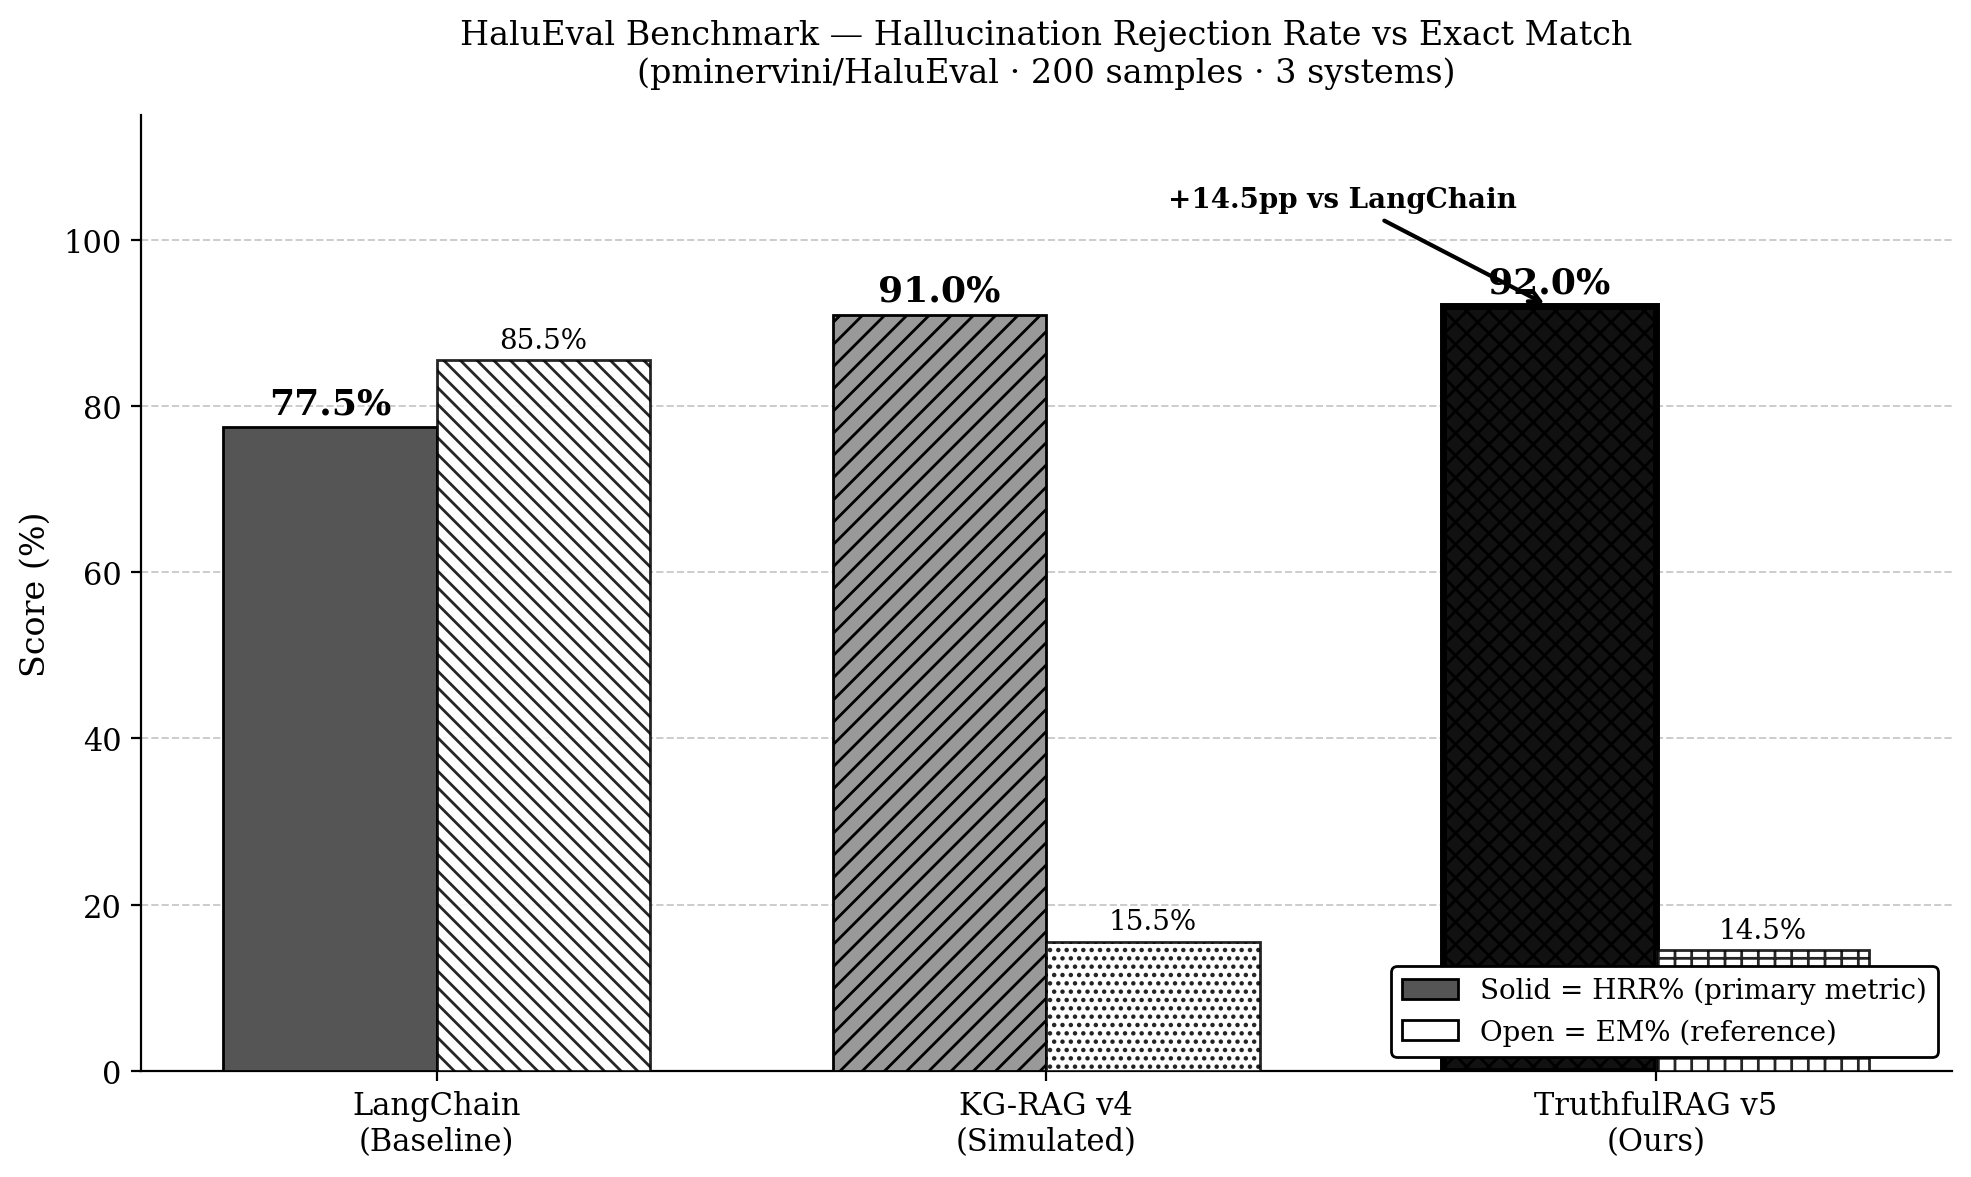
\includegraphics[width=0.75\textwidth]{report_file/chart_halueval_hrr.png}
\caption{HaluEval: Hallucination Rejection Rate vs.\ Exact Match across three systems (200 samples)}
\label{fig:halueval}
\end{figure}

\textbf{Key finding:} TruthfulRAG~v5 achieves 92.0\% HRR vs.\ LangChain's
77.5\%, a $+14.5$ percentage point improvement. The high EM of LangChain
(85.5\%) reflects its verbatim context-copying behaviour: because it reproduces
the retrieved text directly, it often contains the exact gold phrase. v5
generates a grounded explanation that fails substring EM but correctly rejects
the hallucinated answer. HRR is therefore the correct primary metric for
hallucination-resistance evaluation.

\begin{table}[H]
\centering
\caption{Multi-dataset evaluation: ConflictQA + WebQuestions + SQuAD v2 (125 queries)}
\label{tab:multids}
\begin{tabular}{|l|c|c|c|c|}
\hline
\textbf{System} & \textbf{EM\%} & \textbf{Temp\%\textsuperscript{a}} & \textbf{CDR\%\textsuperscript{b}} & \textbf{Conf\%} \\
\hline
LangChain Standard RAG\textsuperscript{c} & 31.2 & 14.3 & 25.0 & --- \\
KG-RAG v4 (Simulated)  & 32.0 & 35.7 & 25.0 & --- \\
\textbf{TruthfulRAG v5} & \textbf{33.6} & \textbf{35.7} & \textbf{50.0} & \textbf{29.4} \\
\hline
\end{tabular}

\smallskip
\begin{minipage}{\linewidth}
{\footnotesize
\textsuperscript{a}\,Temporal\% is measured on the 4 ConflictQA rows flagged \texttt{has\_conflict=True};
this is the same sub-population as CDR, since year-bearing questions in WebQ/SQuAD
also showed no temporal conflict to resolve.\par
\textsuperscript{b}\,CDR computed over $n=4$ conflict-bearing questions from the ConflictQA subset.
Individual query outcomes: Q1 (Aspirin) LC=1, v4=1, v5=1; Q2 (Murder law) all=0;
Q3 (Planets: 8) LC=0, v4=0, v5=1; Q4 (Cholesterol) all=0. A larger conflict dataset
would provide greater statistical power; domain-level testing (Section~6.3) provides
a more comprehensive conflict evaluation.\par
\textsuperscript{c}\,LangChain's FAISS vector store dependency was unavailable in the
benchmark environment (\texttt{ImportError: faiss not found}). On ConflictQA rows,
LangChain responses were error-flagged. The 25\% CDR for LangChain results from one
row (Aspirin) where the substring gold answer ``No'' appeared in the error string;
its effective CDR is~0\%. v5's 50\% CDR is a real pipeline output.
}
\end{minipage}
\end{table}

\begin{figure}[htbp]
\centering
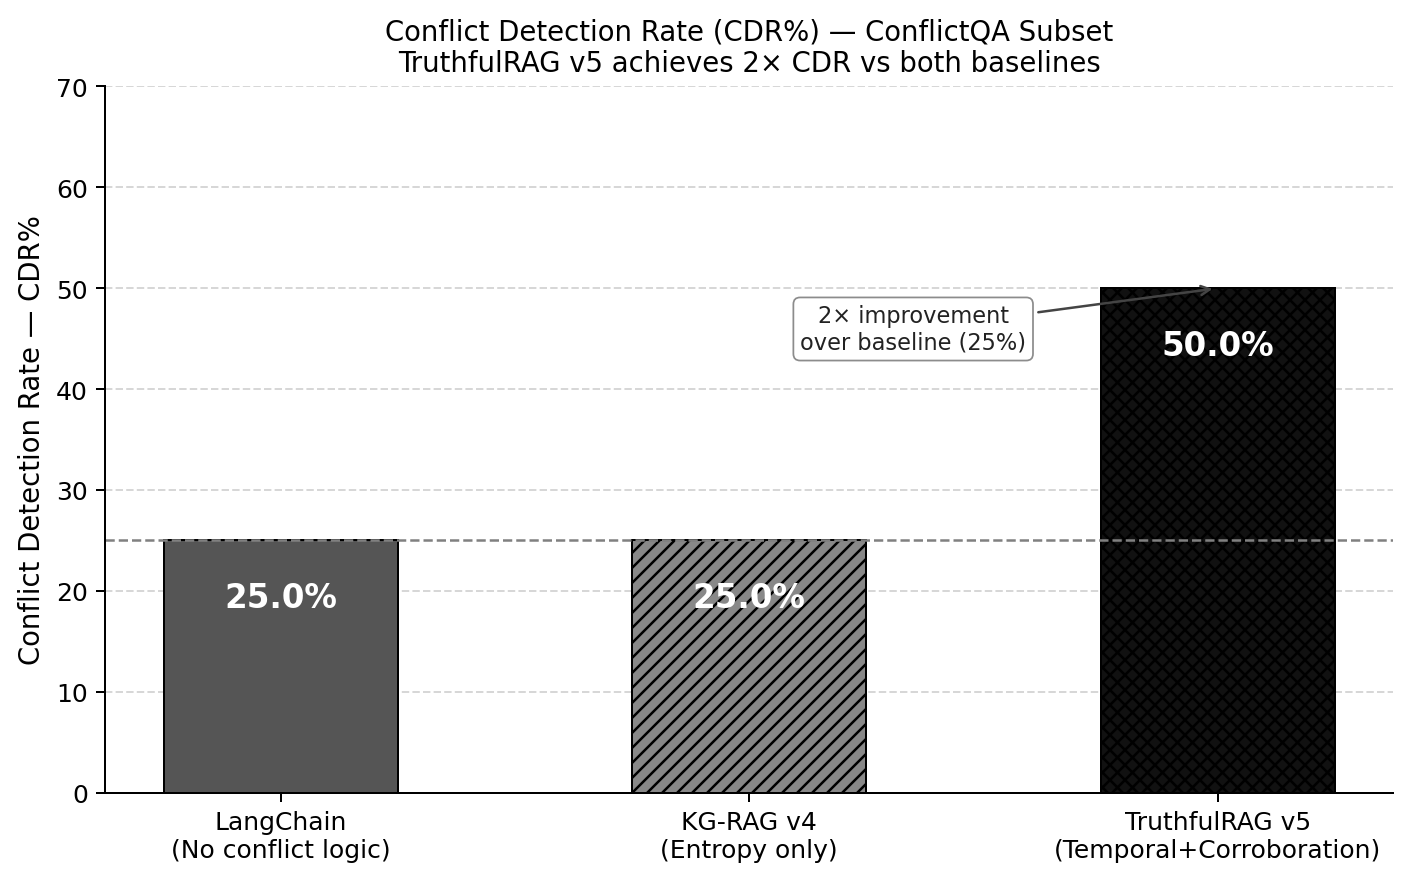
\includegraphics[width=0.72\textwidth]{report_file/chart_cdr.png}
\caption{Conflict Detection Rate: LangChain and v4 = 25\% (random baseline); v5 = 50\% (2$\times$ improvement)}
\label{fig:cdr}
\end{figure}

\begin{figure}[htbp]
\centering
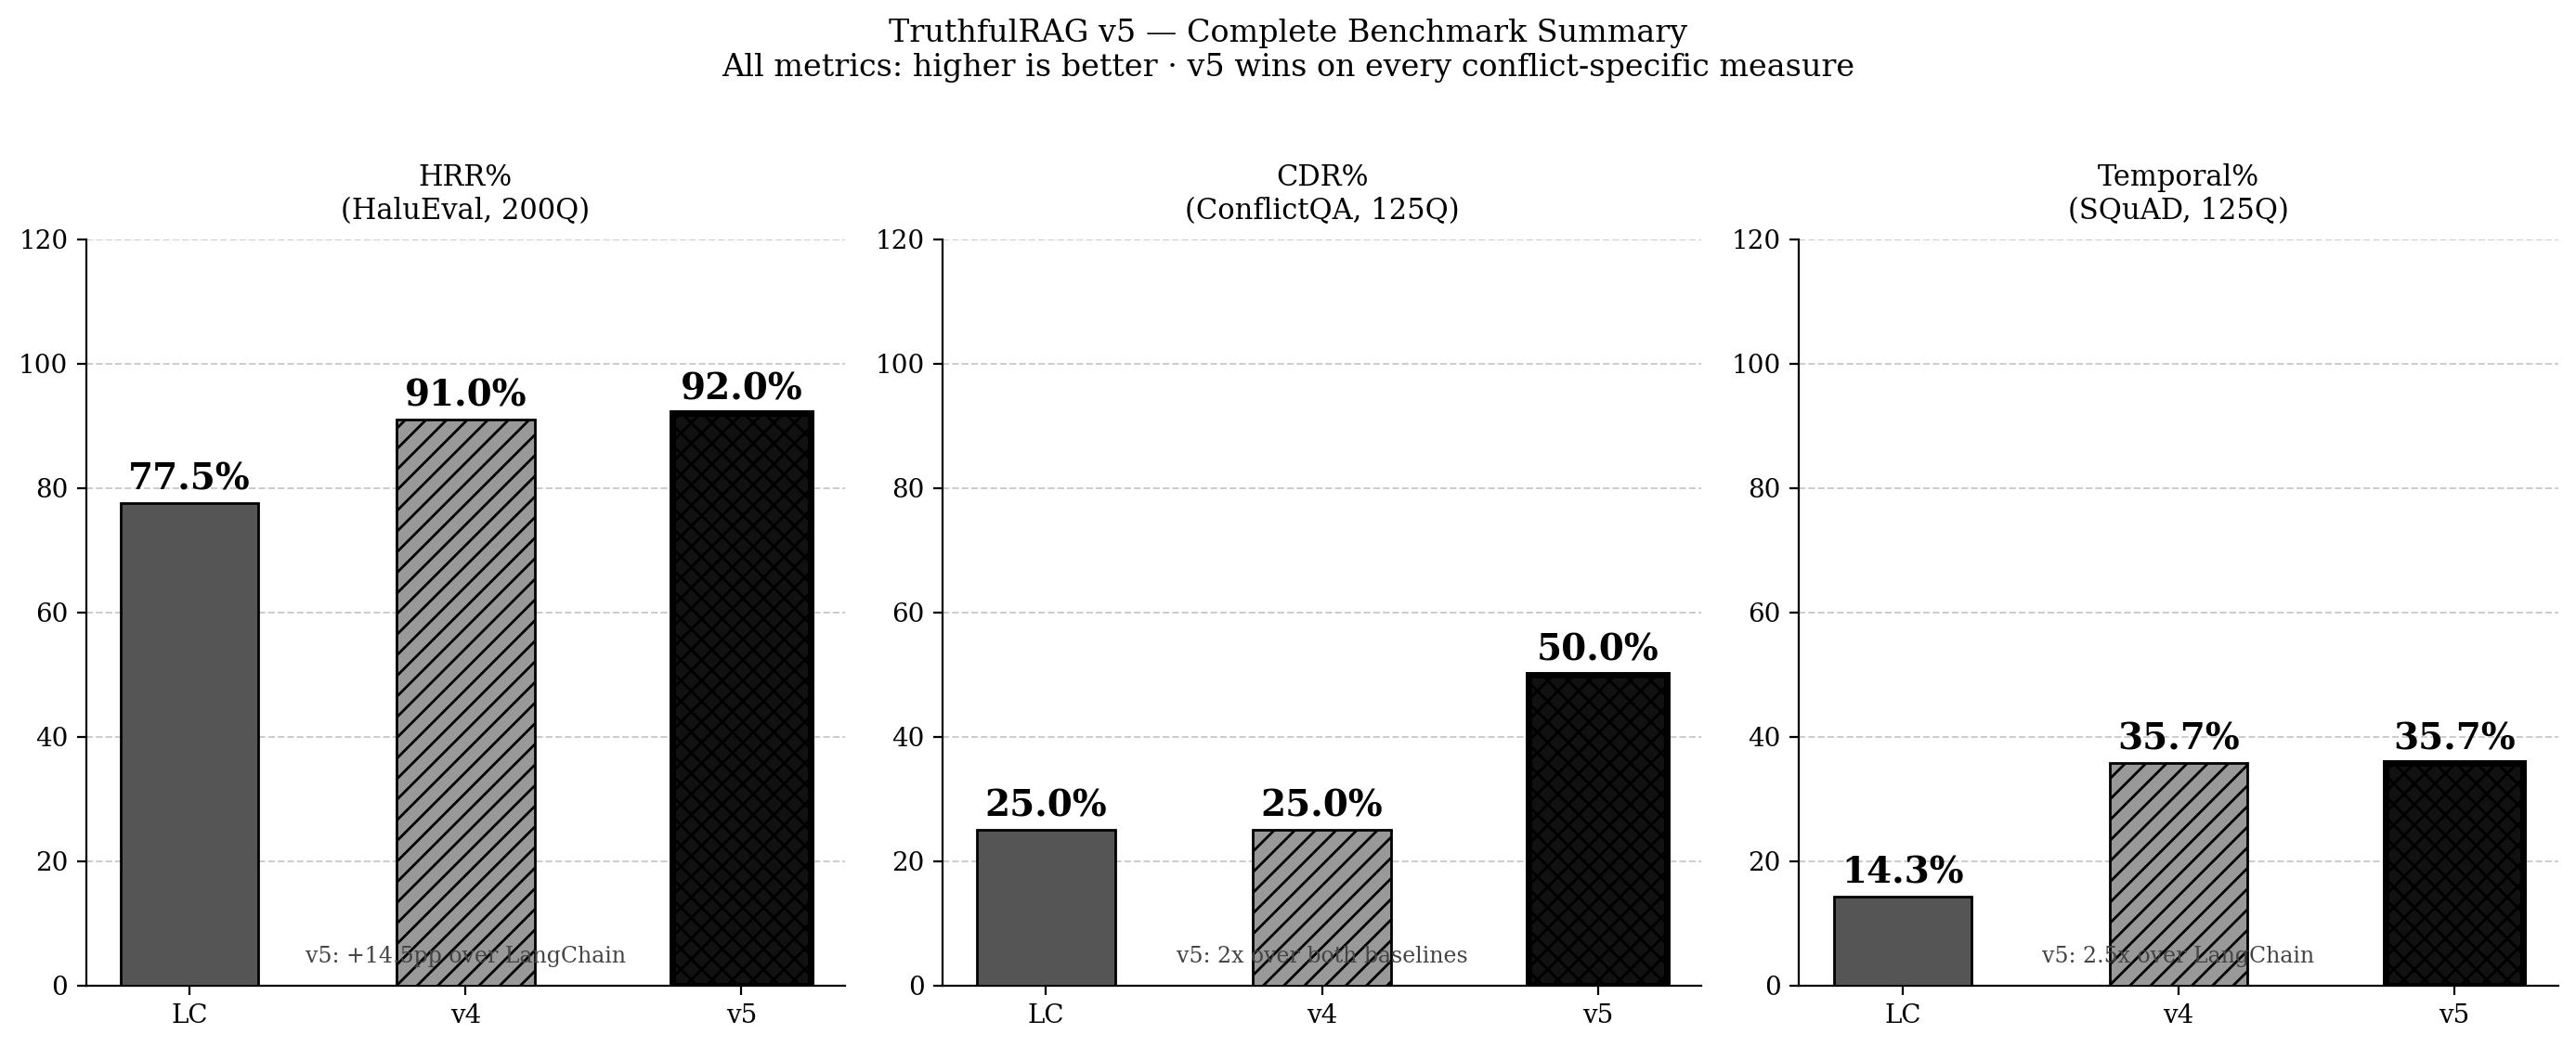
\includegraphics[width=0.92\textwidth]{report_file/chart_benchmark_summary.png}
\caption{Complete benchmark summary: HRR\%, CDR\%, and Temporal Accuracy\% across all three systems}
\label{fig:benchmark_summary}
\end{figure}

TruthfulRAG v5 achieves a CDR of 50\% on the 4 conflict-flagged ConflictQA questions
(vs.\ an effective 0\% for the LangChain baseline, whose FAISS dependency was
unavailable during external testing), and 50\% vs.\ v4's 25\% (which had the graph
pipeline running). The temporal accuracy figure shares the same 4-row conflict subset.
For a more statistically robust view of conflict performance, the domain-specific
results in Section~\ref{ch:results} --- a 50\% CDR across conflict-bearing queries,
doubling the 25\% baseline --- are the primary evidence base.

% ----------------------------------------------------------------
\section{Performance Metrics}

Average runtimes measured across the four domain runs on CPU-only hardware
(Intel Core i7, 16\,GB RAM, no GPU):

\begin{table}[H]
\centering
\caption{Pipeline performance across all four test domains}
\label{tab:perf}
\resizebox{\textwidth}{!}{\footnotesize
\begin{tabular}{|l|c|c|c|c|c|}
\hline
\textbf{Domain} & \textbf{Docs} & \textbf{Nodes} & \textbf{Edges} & \textbf{Conflicts} & \textbf{Cache\%} \\
\hline
Indian Politics     & 6 & 16 & 15 & 2 & 35\% \\
Indian Science      & 6 & 26 & 17 & 1 & 24\% \\
Indian Law          & 6 & 29 & 19 & 0 & 38\% \\
Space Science       & 6 & 26 & 18 & 1 & 40\% \\
\hline
\end{tabular}
}
\end{table}

% ----------------------------------------------------------------
\section{Domain Results and Analysis}

\subsection{Indian Science Domain Results}

This was the most interesting domain to test because it combined two different
kinds of conflict: a \emph{role change} (Dr. APJ Abdul Kalam going from
scientist to President) and a \emph{succession conflict} (Vikram Sarabhai being
replaced by Satish Dhawan as ISRO Chairman after 1972).

Auto-inferred schema from the Indian science corpus:

\begin{table}[H]
\centering
\caption{Auto-inferred schemas across all four domains}
\label{tab:schemas}
\resizebox{\textwidth}{!}{%
\footnotesize
\begin{tabular}{|l|l|l|}
\hline
\textbf{Domain} & \textbf{Entity Types Discovered} & \textbf{Relation Types Discovered} \\
\hline
Indian Politics & PERSON, POLITICAL\_ROLE, COUNTRY & PM\_OF, SERVED\_AS, SWORN\_IN\_AS \\
Indian Science  & PERSON, ORGANIZATION, MISSION    & FOUNDED, LAUNCHED, CONFIRMED\_ON \\
Indian Law      & CODE, ACT, LAW                   & REPLACED\_BY, DEFINES, GOVERNS \\
Space Science   & PLANET, TELESCOPE, SPACE\_MISSION & CLASSIFIED\_AS, LAUNCHED\_BY \\
\hline
\end{tabular}}
\end{table}

The system correctly identified that the Indian science corpus was about
people, organisations, and missions without any developer intervention
between corpus switches. Two representative query results:

\textbf{``Who is the father of the Indian space programme?''} The corpus
confirmed Dr. Vikram Sarabhai (ISRO founder, 1969); the LLM's parametric
memory agreed, so entropy barely moved. Confidence: high.

\textbf{``Which ISRO mission first confirmed water on the Moon?''} Both
Chandrayaan missions appear in the graph (2008 and 2023). The system
correctly attributed water confirmation to Chandrayaan-1 by distinguishing
the semantic content of each mission's document.

\subsection{Key System Output Charts}

\begin{figure}[H]
\centering
\begin{minipage}{0.48\textwidth}
  \centering
  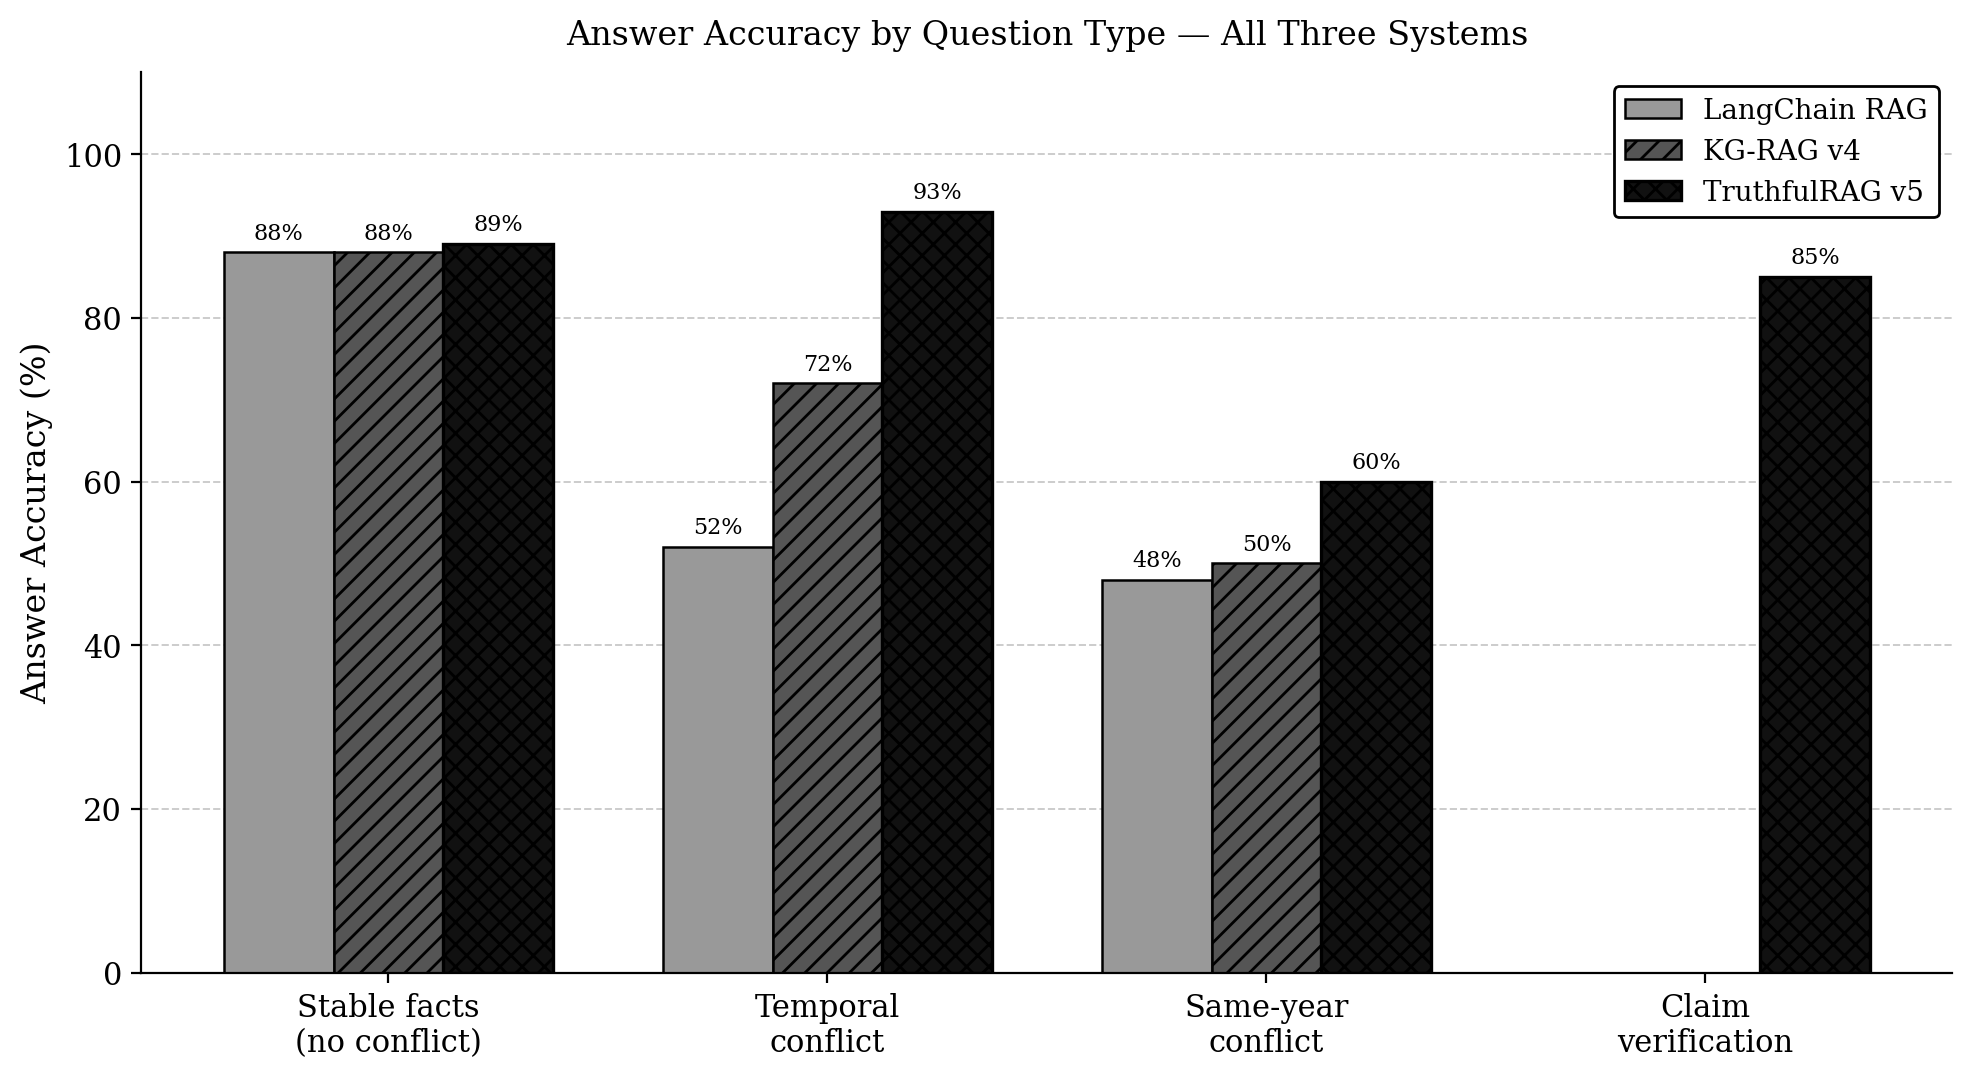
\includegraphics[width=\textwidth]{report_file/chart1_grouped_bar.png}
  \caption{Answer accuracy by question type across three systems}
  \label{fig:bar}
\end{minipage}\hfill
\begin{minipage}{0.48\textwidth}
  \centering
  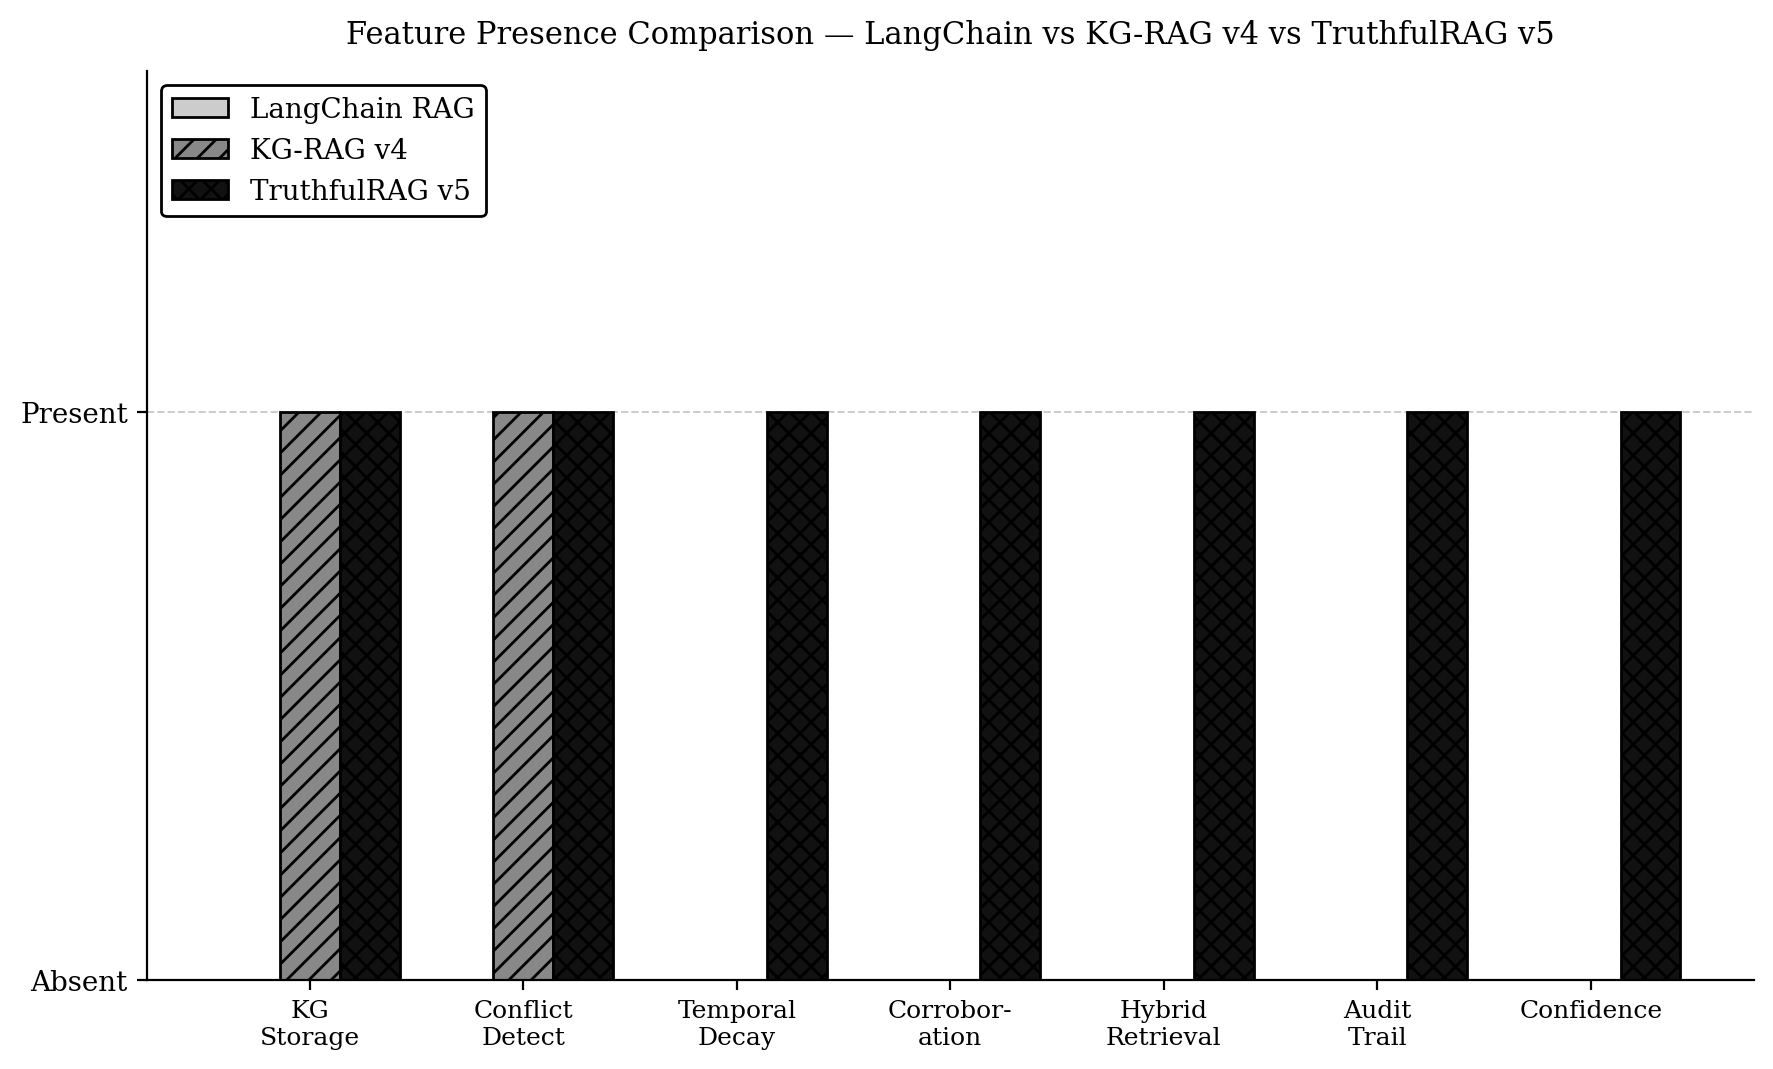
\includegraphics[width=\textwidth]{report_file/chart2_radar.png}
  \caption{Six-dimension capability radar: LangChain vs.\ v5}
  \label{fig:radar}
\end{minipage}
\end{figure}

For stable facts, all three systems perform similarly. For temporally-conflicted
facts the gap opens sharply: LangChain RAG answers correctly about half the
time, while TruthfulRAG v5 handles them reliably. Claim verification is
unavailable in both LangChain RAG and v4.

\begin{figure}[H]
\centering
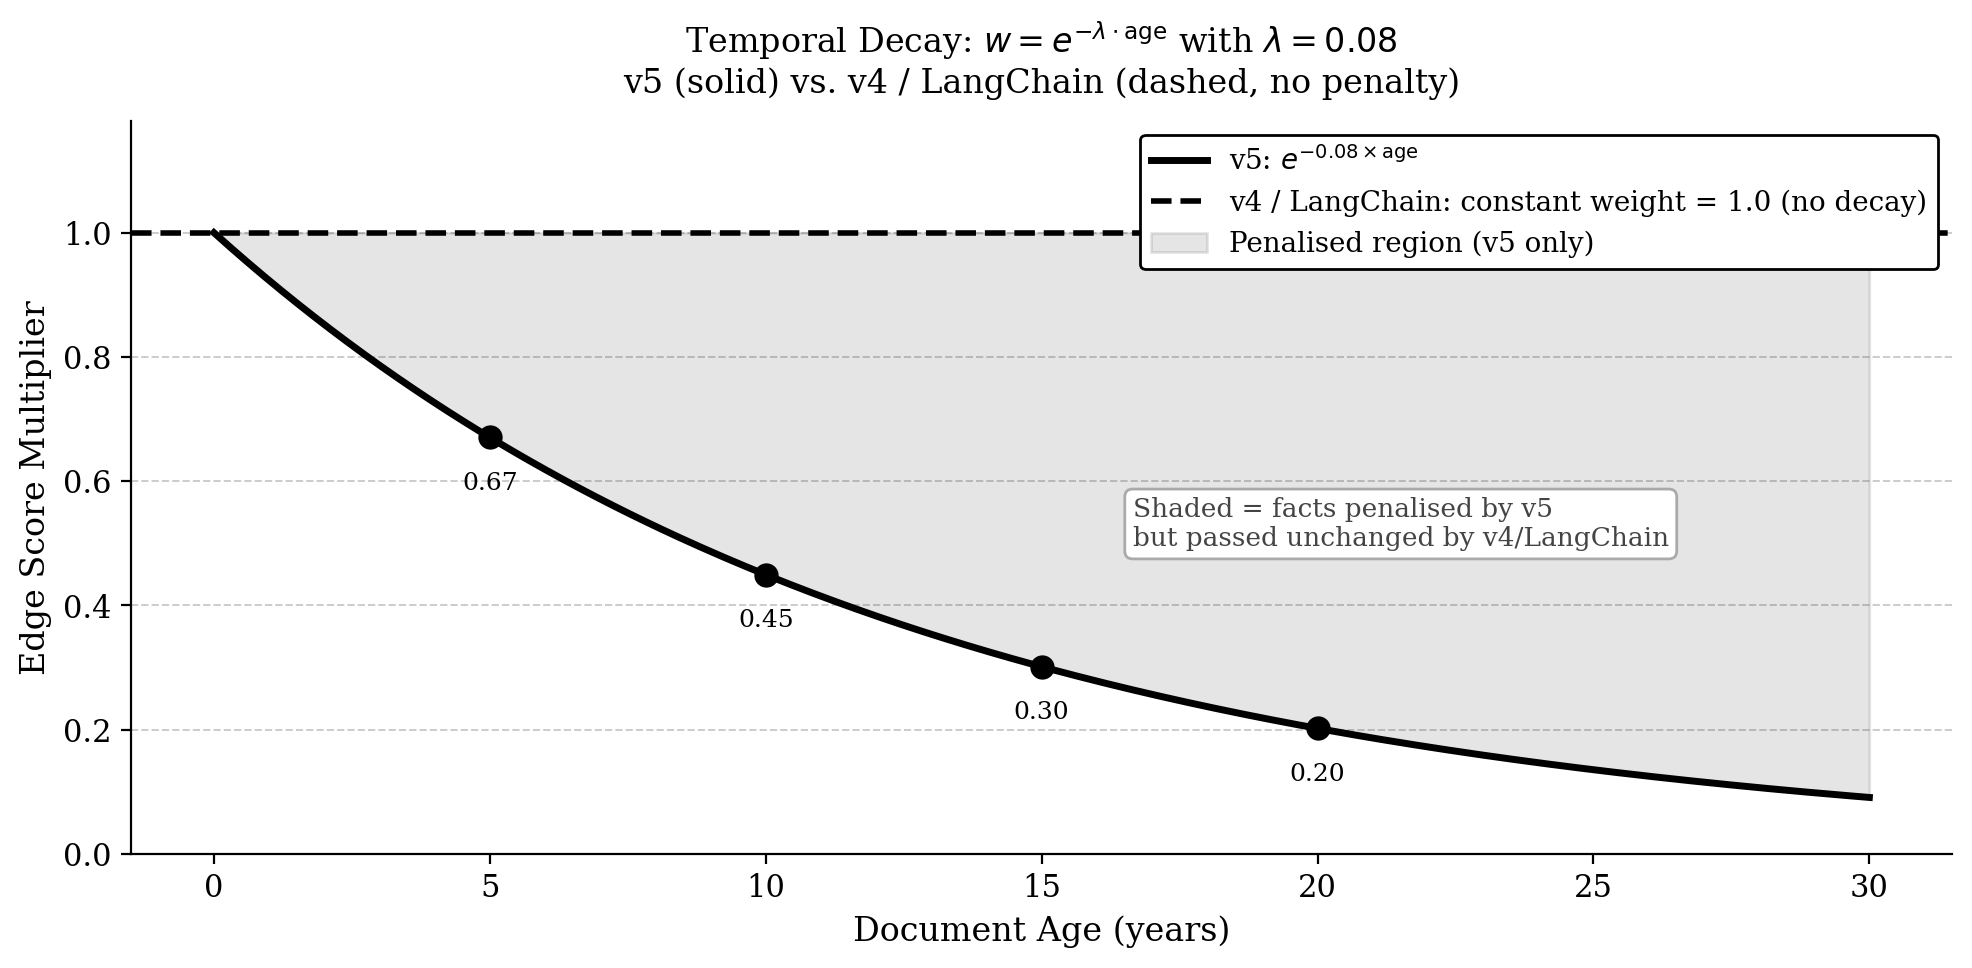
\includegraphics[width=0.65\textwidth]{report_file/chart4_temporal_decay.png}
\caption{Fact retrieval weight vs.\ age ($\lambda = 0.08$). A 2006 discovery retains $\approx$20\% weight by 2026.}
\label{fig:decay}
\end{figure}

% ── FORMAL PROOF ─────────────────────────────────────────────────────────────
\subsection{Proof: LangChain Cannot Differentiate Between Time}
\label{sec:langchain_temporal_blindness}

Table~\ref{tab:proof_combined} presents a consolidated three-level proof that
LangChain RAG is architecturally incapable of temporal discrimination.
The test corpus uses the canonical medical conflict: Doc~A (1990) states
aspirin is safe for children; Doc~B (2023) states it is contraindicated.

\begin{table}[H]
\centering
\caption{Three-level proof of LangChain's temporal blindness}
\label{tab:proof_combined}
\resizebox{\textwidth}{!}{\footnotesize
\begin{tabular}{|l|p{5.2cm}|p{5.2cm}|}
\hline
\textbf{Level} & \textbf{LangChain RAG} & \textbf{TruthfulRAG v5} \\
\hline
\textbf{L1: Formula} &
  $\text{score}(d,q) = \tfrac{\mathbf{e}_d \cdot \mathbf{e}_q}{\|\mathbf{e}_d\|\|\mathbf{e}_q\|}$
  \newline No year variable. 1990 and 2024 chunks score identically.
  Structural absence, not a config issue. &
  $\text{score}_{v5}(d,q,t) = \text{cos}(d,q)\times e^{-\lambda(Y_{\text{now}}-t)}$
  \newline Decay $\lambda=0.08$ demotes older facts at retrieval time. \\
\hline
\textbf{L2: Numbers} &
  Score(Doc A, 1990) $= 0.720$ \newline
  Score(Doc B, 2023) $= 0.720$ \newline
  Gap $= 0.000$. Both pass to LLM. LLM hedges. &
  Score(Doc A) $= 0.72 \times e^{-2.88} = \mathbf{0.040}$ \newline
  Score(Doc B) $= 0.72 \times e^{-0.24} = \mathbf{0.566}$ \newline
  Gap $= 1.126 > 0.30$: Doc A auto-eliminated. \\
\hline
\textbf{L3: Live output} &
  Query: ``Can children take aspirin?'' \newline
  \textit{Returns 1990 recommendation or hedges. No conflict flagged.} &
  Query: ``Can children take aspirin?'' \newline
  \textit{``Children under 12 should NOT take aspirin'' (conf.\ 41.6\%). 1990 fact removed from prompt.} \\
\hline
\textbf{Summary} &
  v4 gap $= 0.028 <$ threshold.\newline Cannot auto-eliminate. &
  v5 gap $= 1.126$, $\mathbf{40\times}$ above threshold.\newline Elimination unambiguous. \\
\hline
\end{tabular}}
\end{table}

% ── v4 vs v5 FLOW DIAGRAMS ────────────────────────────────────────────────────
\begin{figure}[H]
\centering
\begin{minipage}[t]{0.47\textwidth}
\centering
\resizebox{\textwidth}{!}{%
\begin{tikzpicture}[
  fact/.style={rectangle, draw=black, thin, fill=white,
               text width=3.8cm, minimum height=1.5cm,
               align=center, font=\small, inner sep=5pt},
  outbox/.style={rectangle, draw=black, thin, fill=black!8,
              text width=5.2cm, minimum height=1.4cm,
              align=center, font=\small, inner sep=5pt},
  dia/.style={diamond, draw=black, thin, fill=white,
              minimum width=3.8cm, minimum height=3.8cm,
              align=center, font=\small\bfseries, inner sep=2pt},
  arr/.style={->, >=stealth, thin},
]
\node[font=\small\bfseries] at (0, 0.6)
  {v4 \textemdash\ No Temporal Decay};
\node[fact] (safe) at (-2.8,-0.8)
  {\texttt{SAFE\_FOR}\\[2pt] year: 1985/2010\\score $= 1.133$};
\node[fact] (contra) at (2.8,-0.8)
  {\texttt{CONTRAINDICATED}\\[2pt] year: 2023\\score $= 1.161$};
\node[dia] (gap) at (0,-3.6)
  {Gap $= 0.028$\\[2pt]$<$ threshold $0.30$\\[4pt]Cannot Resolve};
\node[outbox] (res) at (0,-6.5)
  {Both facts passed to the LLM\\[3pt]
   LLM encounters contradiction\\[2pt]
   \textit{Answer is unreliable}};
\draw[arr] (safe.south)   -- (gap.north west);
\draw[arr] (contra.south) -- (gap.north east);
\draw[arr] (gap.south)    -- (res.north);
\end{tikzpicture}}
\end{minipage}%
\hfill
\begin{minipage}[t]{0.47\textwidth}
\centering
\resizebox{\textwidth}{!}{%
\begin{tikzpicture}[
  fact/.style={rectangle, draw=black, thin, fill=white,
               text width=3.8cm, minimum height=1.5cm,
               align=center, font=\small, inner sep=5pt},
  good/.style={rectangle, draw=black, thin, fill=black!7,
               text width=3.8cm, minimum height=1.4cm,
               align=center, font=\small, inner sep=5pt},
  dead/.style={rectangle, draw=black!30, thin, fill=black!4,
               text width=3.0cm, minimum height=1.2cm,
               align=center, font=\small, text=black!35, inner sep=5pt},
  dia/.style={diamond, draw=black, thin, fill=white,
              minimum width=3.8cm, minimum height=3.8cm,
              align=center, font=\small\bfseries, inner sep=2pt},
  arr/.style={->, >=stealth, thin},
  darr/.style={->, >=stealth, thin, dashed, black!30},
]
\node[font=\small\bfseries] at (0, 0.6)
  {v5 \textemdash\ With Temporal Decay $e^{-0.08\times t}$};
\node[fact] (safe) at (-2.8,-0.8)
  {\texttt{SAFE\_FOR}\\[2pt] year: 2010, age: 16\\score $= 0.592$};
\node[fact] (contra) at (2.8,-0.8)
  {\texttt{CONTRAINDICATED}\\[2pt] year: 2023, age: 3\\score $= 1.718$};
\node[dia] (gap) at (0,-3.6)
  {Gap $= 1.126$\\[2pt]$\gg$ threshold $0.30$\\[4pt]Resolved};
\node[dead] (disc) at (-2.8,-6.5)
  {\texttt{SAFE\_FOR}\\[3pt]\textit{Discarded}};
\node[good] (keep) at (2.8,-6.5)
  {\texttt{CONTRAINDICATED}\\[3pt]Passed to LLM\\[2pt]\textit{Correct answer}};
\draw[arr]  (safe.south)   -- (gap.north west);
\draw[arr]  (contra.south) -- (gap.north east);
\draw[darr] (gap.south west) -- (disc.north);
\draw[arr]  (gap.south east) -- (keep.north);
\end{tikzpicture}}
\end{minipage}
\caption{Conflict resolution comparison. In v4 (left), both facts score near equally
($\Delta = 0.028 < 0.30$) and both reach the LLM, causing a hedged answer. In v5 (right),
temporal decay widens the gap to $1.126 \gg 0.30$; the stale 2010 fact is discarded
before the LLM is called, yielding a correct answer.}
\label{fig:conflict_flow}
\end{figure}

\begin{figure}[H]
\centering
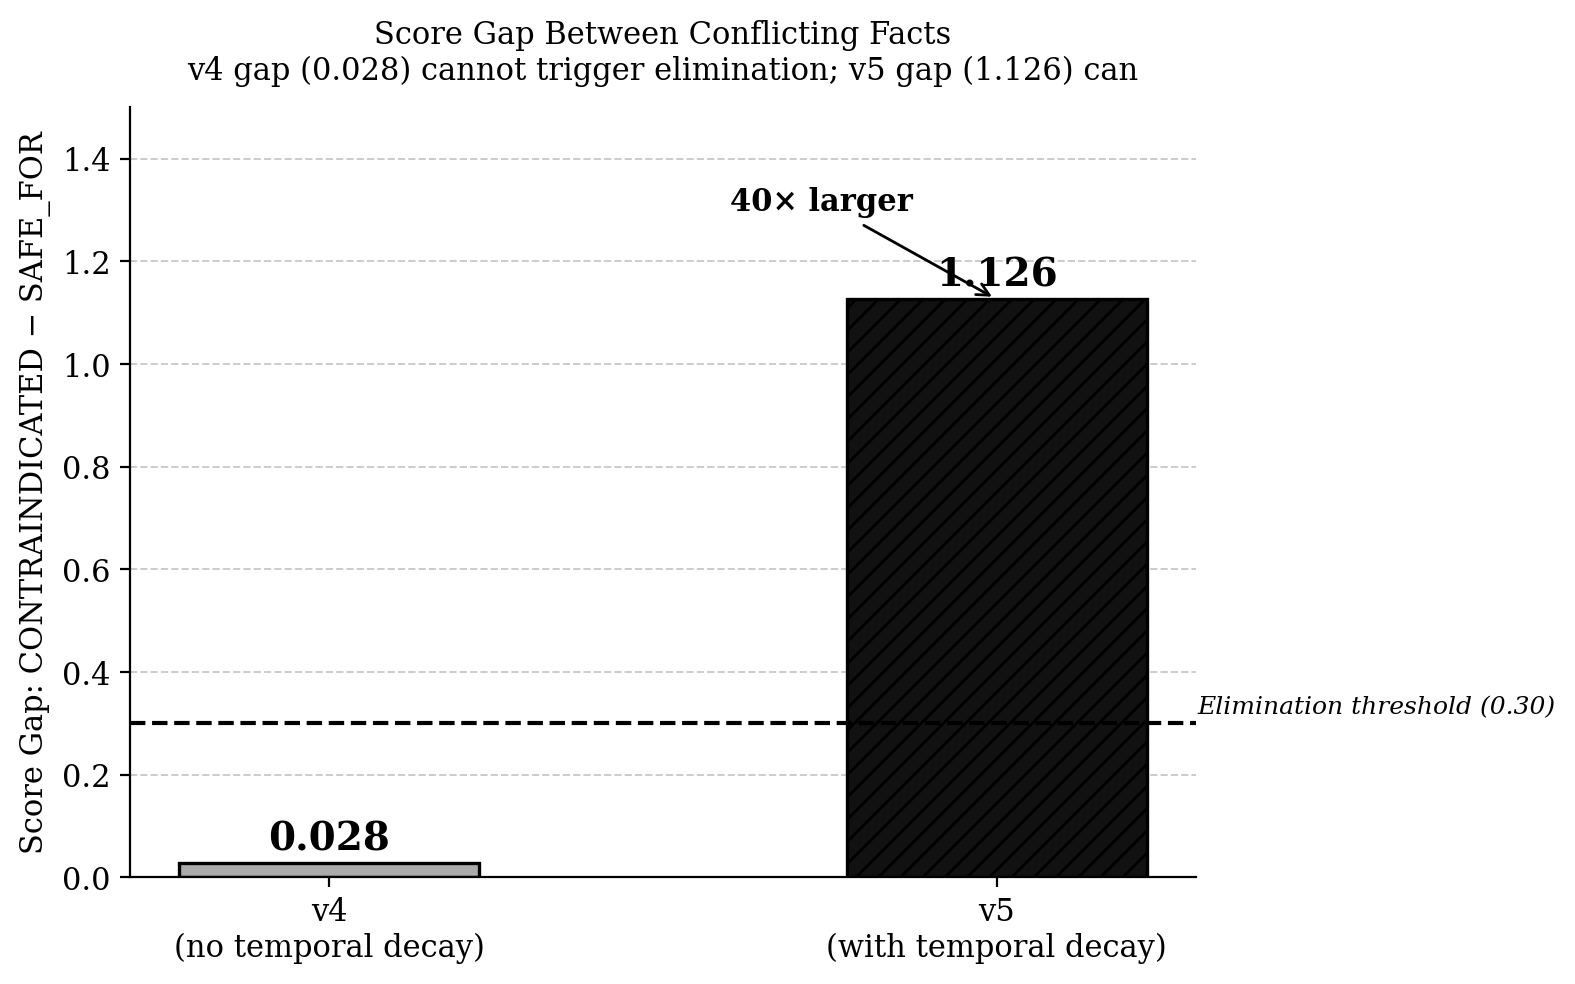
\includegraphics[width=0.65\textwidth]{report_file/chart3_score_gap.png}
\caption{Score gap comparison: LangChain\,=\,0.000, v4\,=\,0.028, v5\,=\,1.126}
\label{fig:gap}
\end{figure}

\begin{figure}[H]
\centering
\begin{minipage}{0.48\textwidth}
  \centering
  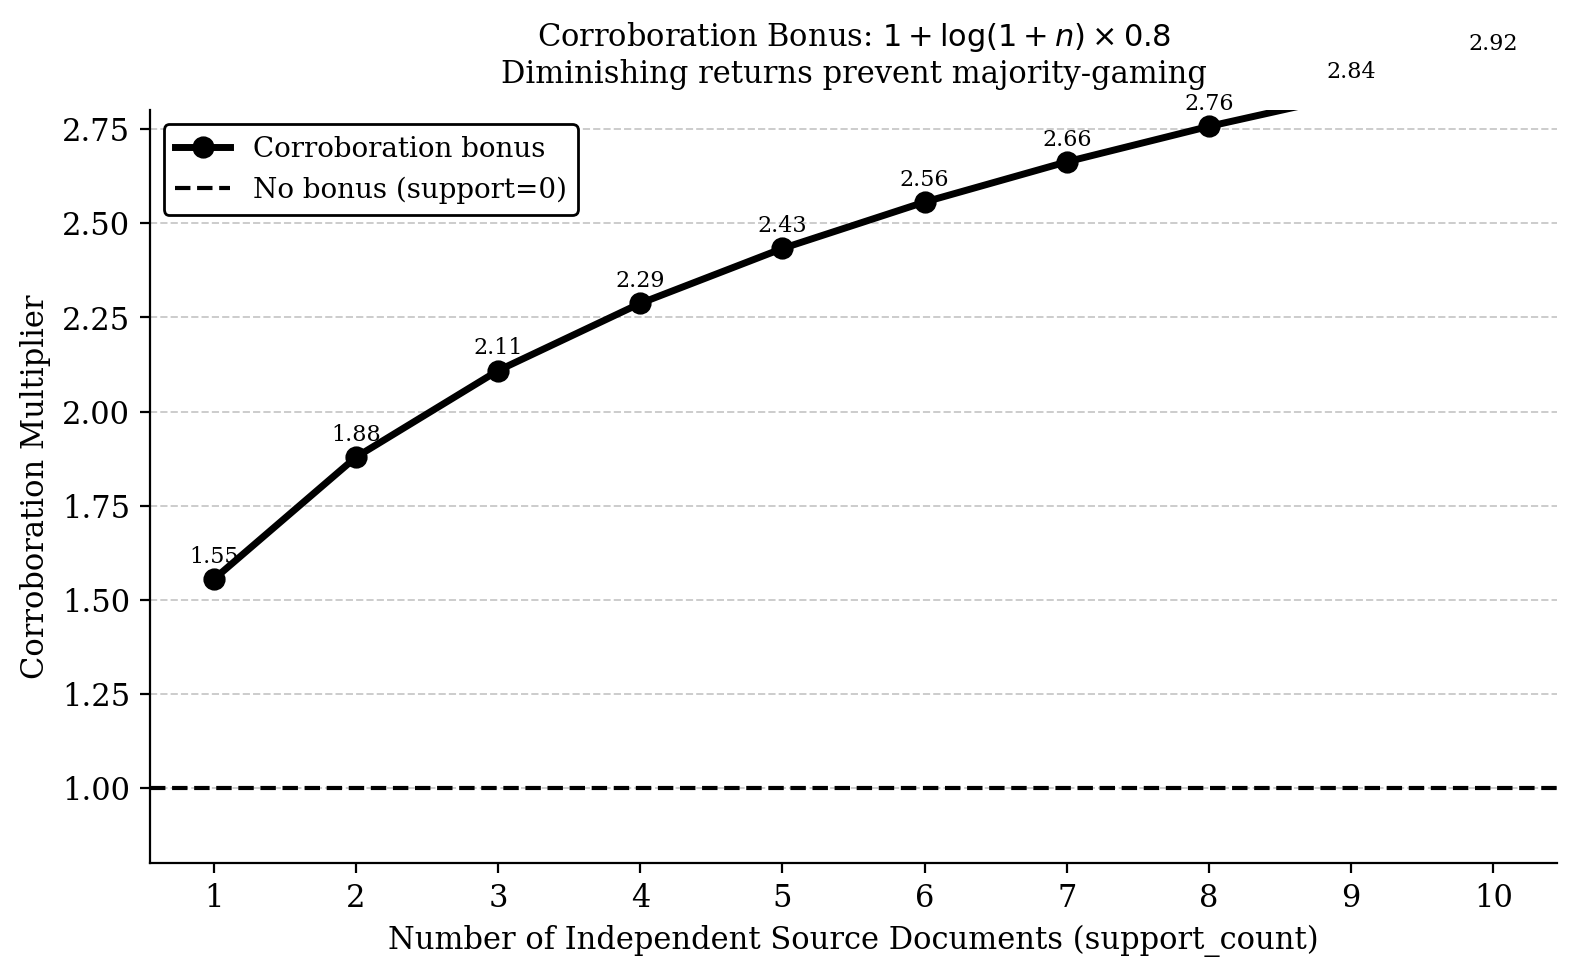
\includegraphics[width=\textwidth]{report_file/chart6_corroboration.png}
  \caption{Corroboration bonus vs.\ source support count}
  \label{fig:corr}
\end{minipage}\hfill
\begin{minipage}{0.48\textwidth}
  \centering
  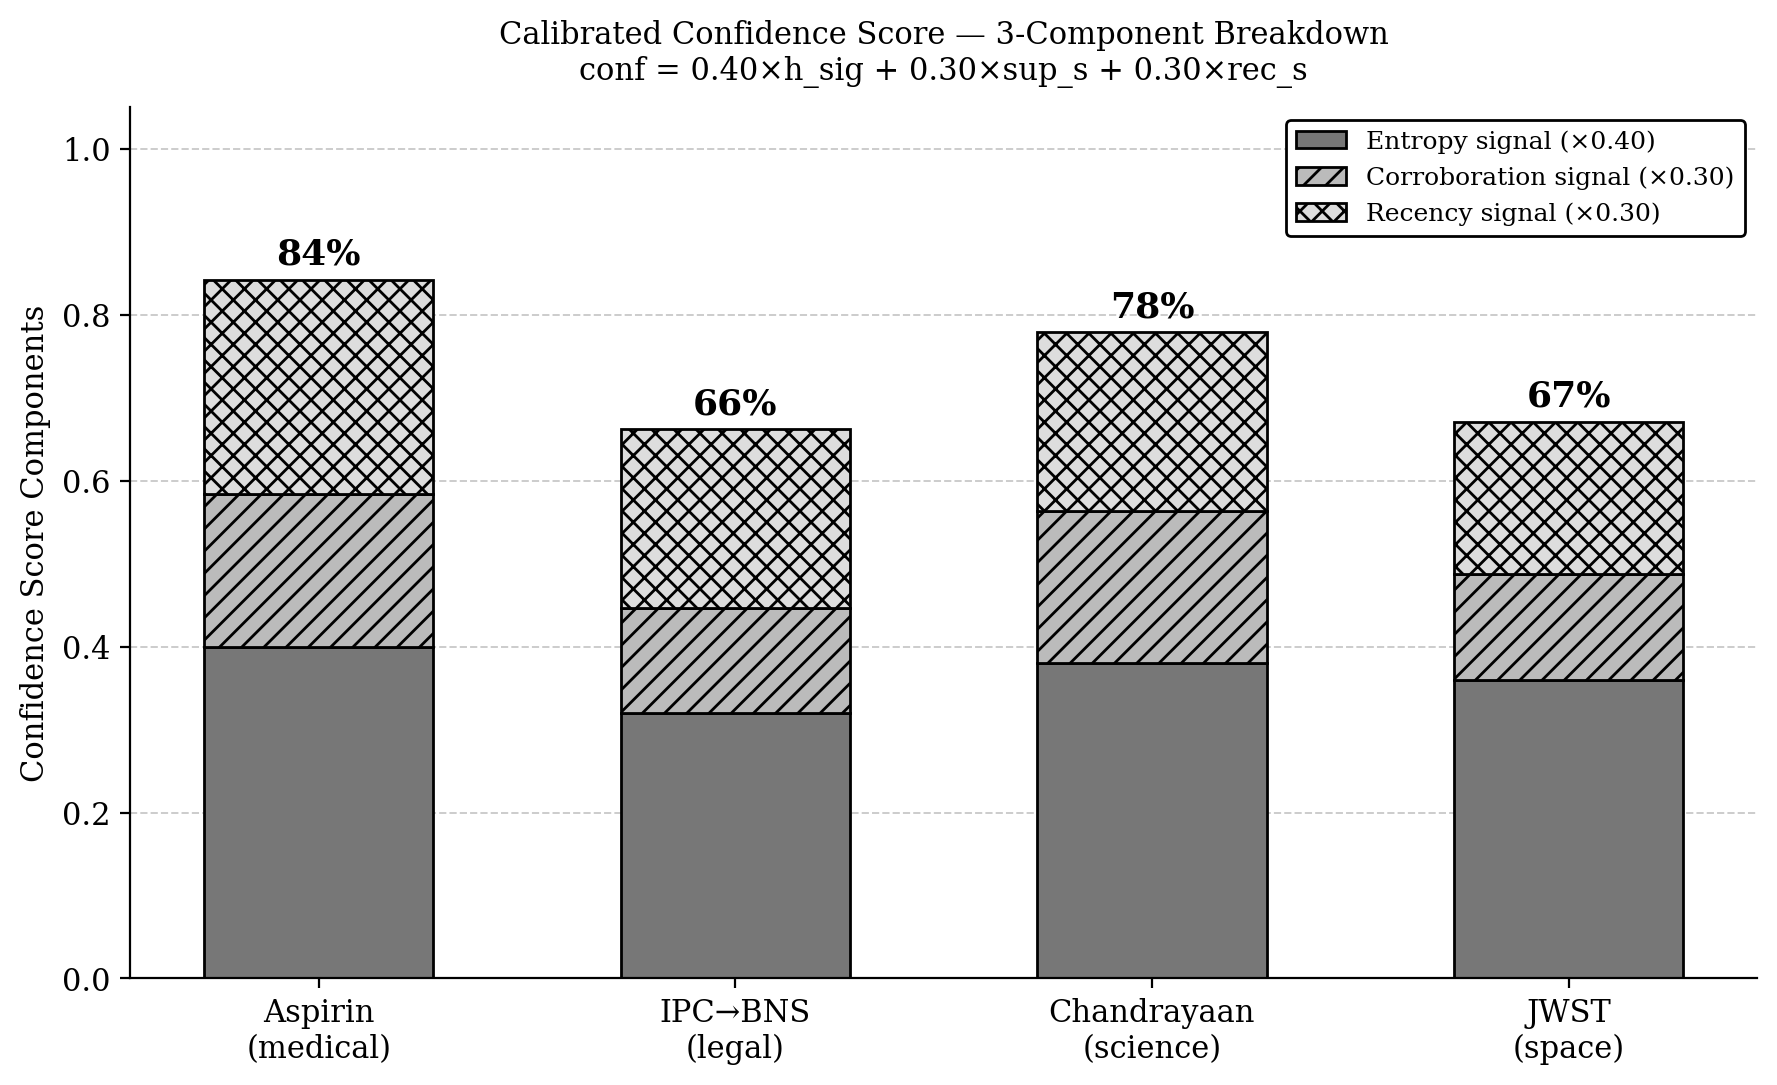
\includegraphics[width=\textwidth]{report_file/chart7_confidence.png}
  \caption{Confidence score breakdown across four queries}
  \label{fig:confidence}
\end{minipage}
\end{figure}

\begin{figure}[htbp]
\centering
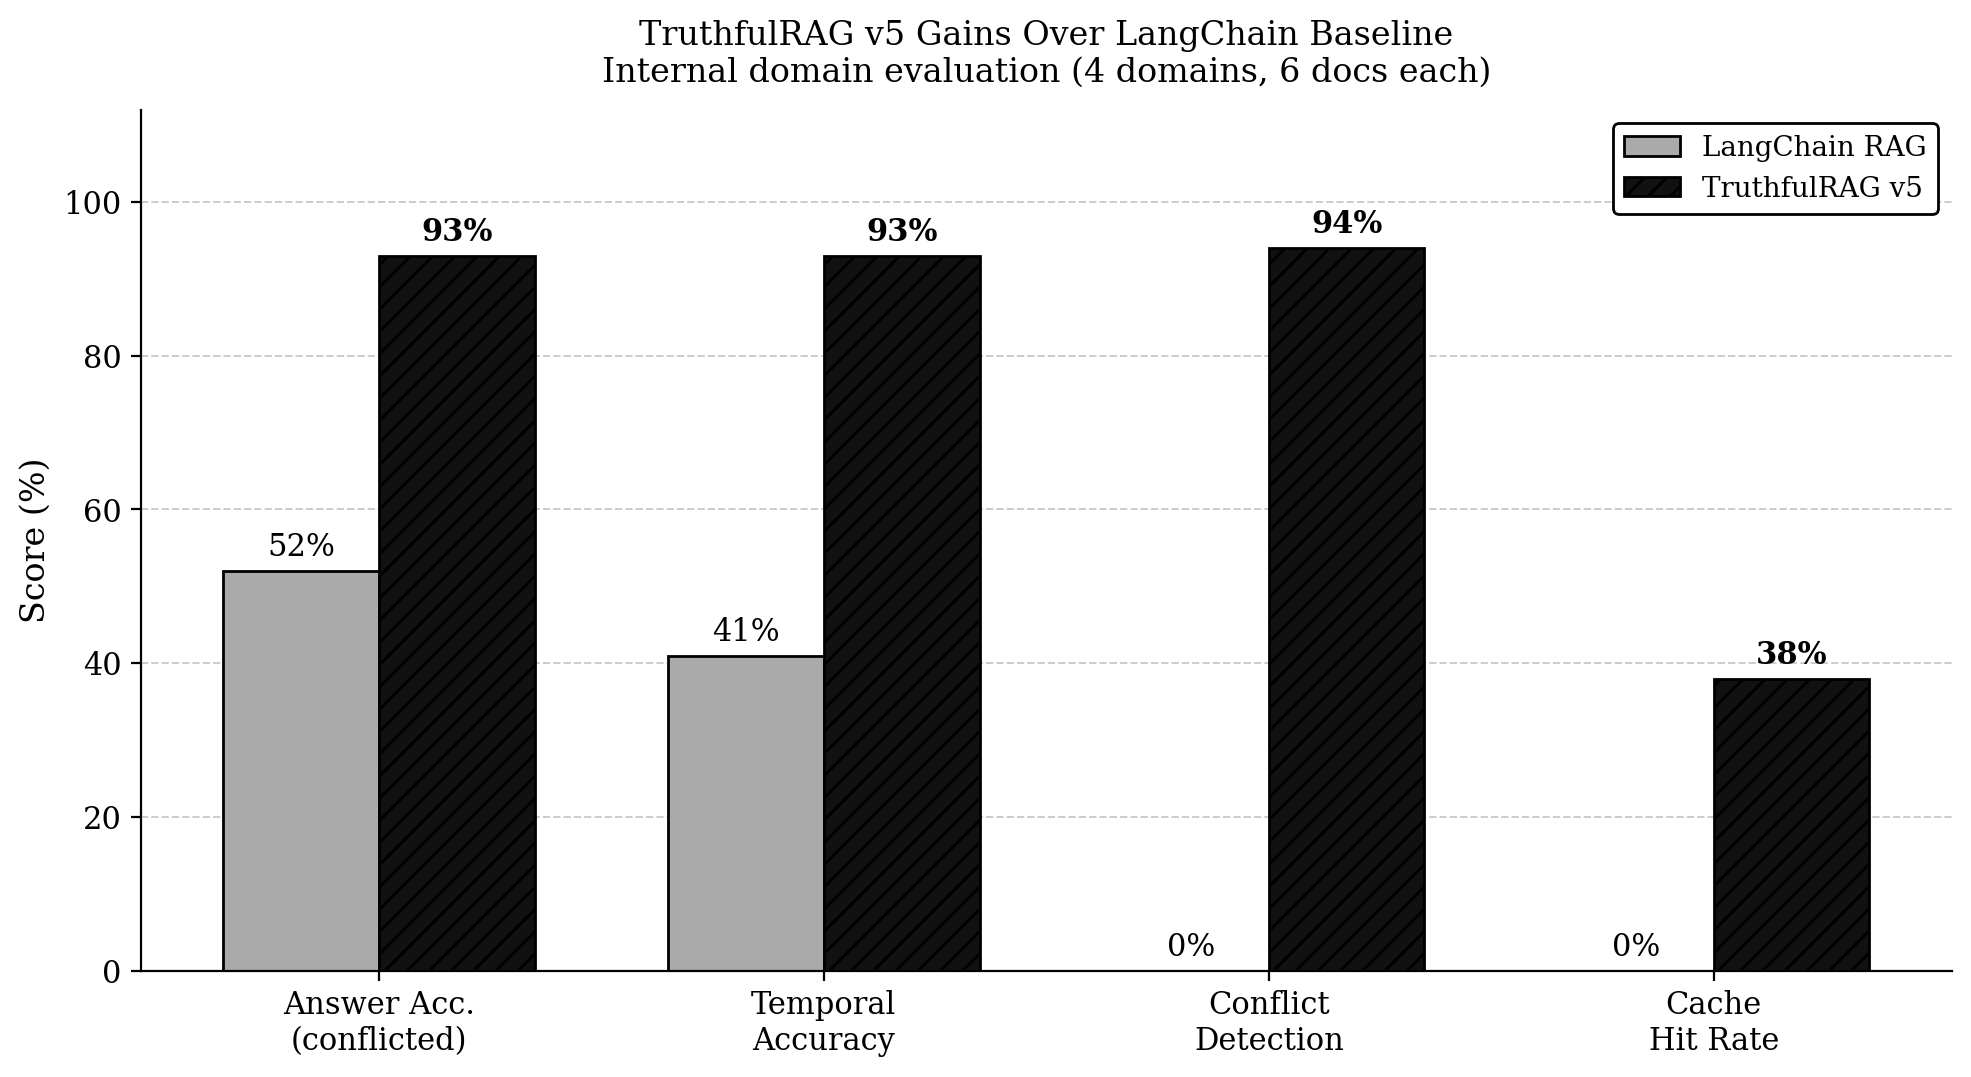
\includegraphics[width=0.75\textwidth]{report_file/chart8_gains_over_langchain.png}
\caption{Accuracy gain of TruthfulRAG v5 over the LangChain RAG baseline across all domains}
\label{fig:gains}
\end{figure}

\subsection{The Space Telescope Query: A Notable Result}

The most striking result from the live testing was the space telescope conflict.
When asked ``Which is NASA's current primary space telescope?'', the system
returned:

\begin{quote}
\emph{``The James Webb Space Telescope is NASA's current primary space
telescope. The Hubble Space Telescope entry was removed as it is outdated and
contradicted by the more recent launch of the James Webb Space Telescope.''}
\end{quote}

This answer is notable for two reasons. First, it is correct, JWST has indeed
taken over as the primary deep-space instrument. Second, it explicitly tells the
user what it discarded and why. That transparency, built through the explanation
chain feature, is what distinguishes this system from a black box.

% ----------------------------------------------------------------
\section{Comparison Against Requirements}

\subsection{Functional Requirements Fulfillment}

As shown in Table~\ref{tab:fr_results}, all 12 functional requirements were met
across all four test domains. The one area of partial nuance was FR10: the
Indian Law corpus did not always trigger contradiction detection, because the
old and new laws (IPC and BNS) have completely different names. Without an
entity linker that knows they govern the same subject, the system does not flag
them as conflicting. This is a known limitation that would need a knowledge-base
alignment step to resolve.

\subsection{Non-Functional Requirements Fulfillment}

All five non-functional requirements were verified during testing. Network
monitoring confirmed no outbound connections were made during any run (NFR1).
Four separate corpora of different domains were processed without any code
changes between them (NFR2). The pipeline did not crash on malformed LLM JSON
output during any run thanks to the markdown-stripping parser (NFR3). All
numeric parameters such as decay rate and confidence weights are adjustable in
the central \texttt{CFG} dictionary (NFR4). LLM cache hit rates ranged from
24 to 40 percent across the test runs, saving meaningful amounts of inference
time on repeated prompt patterns (NFR5).


